\documentclass{beamer}

\usetheme{PATS}
\usepackage[english]{babel}
\usepackage[utf8]{inputenc}
\usepackage[T1]{fontenc}
\usepackage{cmap}
\usepackage{listings}
\usepackage{hyperref}
\setbeamercovered{transparent}

\title{Click Coding}
\subtitle{Coding with Click Modular Router}
\author{Bart Braem \and Johan Bergs}
\institute{University of Antwerp\\iMinds - MOSAIC Research Group}
\date{October 2014}

\logo{
\includegraphics[height=1cm]{figures/pats_logo.jpg}}


\begin{document}

\lstset{breakatwhitespace=true}
\lstset{language=C++}
\lstset{columns=fullflexible}
\lstset{keepspaces=true}
\lstset{breaklines=true,
        tabsize=3, 
        showstringspaces=false,
extendedchars=\true}

\begin{frame}[t]
\titlepage
\end{frame}


\section*{Outline}

\frame{
  \frametitle{Outline}
  \tableofcontents[subsectionstyle=hide]
}

\section{Coding}
\subsection{Writing custom elements} % (fold)
\label{sub:writing_custom_elements}
\frame{
\frametitle{Do it yourself}
Let's make an example element
\begin{itemize}
\item 1 input, 1 output, Push
\item Configure a packet size threshold, if larger: drop packet
\end{itemize}
Download the source code online to avoid copy errors at \url{https://github.com/mosaicresearch/click_modular_router_lessons/tree/master/examples/simpleelements}
}

\begin{frame}[fragile]
\frametitle{Element header}
Necessary in the header:
\begin{itemize}
	\item Include-guard macros
	\item Click element macros
	\item Include click/element.hh
	\item The class declaration containing 3 special methods:
\end{itemize}
\begin{lstlisting}
const char *class_name() const
const char *port_count() const
const char *processing() const
\end{lstlisting}
\end{frame}

\begin{frame}[fragile]
\frametitle{Element header}
Necessary in the source file:
\begin{itemize}
	\item Include \!click/config.hh! \textbf{first}!
	\item \lstinline!CLICK_DECLS! macro
	\item \lstinline!CLICK_ENDDECLS! macro
	\item \lstinline!EXPORT_ELEMENT! macro
	\item Implementation of the methods
\end{itemize}
\end{frame}

\begin{frame}[fragile]
\frametitle{simplepushelement.hh}
\begin{lstlisting}[basicstyle=\scriptsize]
#ifndef CLICK_SIMPLEPUSHELEMENT_HH
#define CLICK_SIMPLEPUSHELEMENT_HH
#include <click/element.hh>

CLICK_DECLS
class SimplePushElement : public Element { 
  public:
    SimplePushElement();
    ~SimplePushElement();
    const char *class_name() const { return "SimplePushElement"; }
    const char *port_count() const { return "1/1"; }
    const char *processing() const { return PUSH; }
    int configure(Vector<String>&, ErrorHandler*);
    void push(int, Packet*);
  private:
    uint32_t maxSize;
};
CLICK_ENDDECLS
#endif
\end{lstlisting}
\end{frame}

\begin{frame}[fragile,allowframebreaks]
\frametitle{simplepushelement.cc}
\begin{lstlisting}[basicstyle=\scriptsize]
#include <click/config.h>
#include <click/confparse.hh>
#include <click/error.hh>
#include "simplepushelement.hh"

CLICK_DECLS
SimplePushElement::SimplePushElement() {}
SimplePushElement::~SimplePushElement() {}

int SimplePushElement::configure(Vector<String> &conf, ErrorHandler *errh) {
  if (cp_va_kparse(conf, this, errh, "MAXPACKETSIZE", cpkM, cpInteger, &maxSize, cpEnd) < 0) return -1;
  if (maxSize <= 0) return errh->error("maxsize should be larger than 0");
  return 0;
}

void SimplePushElement::push(int, Packet *p){
  click_chatter("Got a packet of size %d", p->length());
  if (p->length() > maxSize)  p->kill();
  else output(0).push(p);
}
CLICK_ENDDECLS
EXPORT_ELEMENT(SimplePushElement)
\end{lstlisting}
\end{frame}

\begin{frame}[fragile]
\frametitle{What's in a name}
To avoid confusion, we recommend to:
\begin{itemize}
	\item Make the ElementName CamelCase
	\item Use that name in the \lstinline!class_name! macro
	\item Use that name in lowercase for the header (.hh) and source (.cc) files
	\item Use that name in uppercase, with \lstinline!CLICK_! prepended, for the include guards
\end{itemize}
\end{frame}

\begin{frame}[fragile]
\frametitle{simplepullelement}
\begin{lstlisting}[basicstyle=\scriptsize]
simplepullelement.hh:

class SimplePullElement: public Element { 
  public: ...
    const char *processing() const { return PULL; }
    Packet* pull(int);
}

simplepullelement.cc:

Packet* SimplePullElement::pull(int) {
  Packet* p = input(0).pull();
  if(p == 0) return 0;
  click_chatter("Got a packet of size %d",p->length());
  if (p->length() > maxSize){
    p->kill();
    return 0;
  } else return p;
}
\end{lstlisting}
\end{frame}

\begin{frame}[fragile]
\frametitle{simpleagnosticelement}
\begin{lstlisting}[basicstyle=\footnotesize,emph={AGNOSTIC},emphstyle=\underbar]
simpleagnosticelement.hh:
class SimpleAgnosticElement: public Element { 
  public: ...
    const char *processing() const { return AGNOSTIC; }
    void push(int, Packet *);
    Packet* pull(int);
};

simpleagnosticelement.cc
void SimpleAgnosticElement::push(int, Packet *p) {
  // see push element
}
Packet* SimpleAgnosticElement::pull(int) {
  // see pull element
}
\end{lstlisting}
\end{frame}

\begin{frame}[fragile]
\frametitle{simpleagnosticelement11}
\begin{lstlisting}[basicstyle=\scriptsize, emph={AGNOSTIC,simple_action},emphstyle=\underbar]
simpleagnosticelement11.hh:

class SimpleAgnosticElement11: public Element { 
  public: ...
    const char *processing() const { return AGNOSTIC; }
    const char *port_count() const { return "1/1"; }
    Packet *simple_action(Packet *);
};

simpleagnosticelement11.cc
Packet* SimpleAgnosticElement11::simple_action(Packet *p){
  click_chatter("Got a packet of size %d",p->length());
  if (p->length() > maxSize){
    p->kill();
    return 0;
  } else return p;
}
\end{lstlisting}
\end{frame}

\begin{frame}[fragile]
\frametitle{Port count}
Defined by \lstinline!const char *port_count() const!. Can return:
\begin{itemize}
	\item "1/1": one input port, one output port
	\item "1/2": one input port, two output ports
	\item "1-2/0": one or two input ports and zero output ports. 
	\item "1/-6": One input port and up to six output ports. 
	\item "2-/-": At least two input ports, any number of output ports. 
	\item "3"!: Exactly three input and output ports. (If no slash appears, the text is used for both input and output ranges.) 
	\item "1-/=": At least one input port and the same number of output ports. 
	\item "1-/=+": At least one input port and one more output port than there are input ports.
\end{itemize}
\end{frame}
% subsection writing_custom_elements (end)

% \subsection{Configuration Parsing} % (fold)
% \label{sub:configuration_parsing}

\begin{frame}[fragile,allowframebreaks]
\frametitle{Parsing configurations with cp\_va\_kparse}
Call this function on
\begin{itemize}
	\item the configuration (conf)
	\item the element (this) 
	\item the errorhandler (errh)
	\item an argument list
	\item a closing mark (cpEnd)
\end{itemize}
Check the return value (C-style):
\begin{itemize}
	\item 0: all parsing went fine
	\item Negative: problems detected, configure should return -1
\end{itemize}

\begin{lstlisting}[basicstyle=\footnotesize]
int MyElement::configure(Vector<String> &conf, ErrorHandler *errh) {
  String data;
  uint32_t limit = 0;
  bool stop = false;
  
  if (cp_va_kparse(conf, this, errh, 
    "DATA", cpkP+cpkM, cpString, &data, 
    "LIMIT", cpkP, cpUnsigned, &limit, 
    "STOP", 0, cpBool, &stop, 
    cpEnd) < 0) return -1;
  ...
}
\end{lstlisting}
\end{frame}

\begin{frame}[fragile,allowframebreaks]
\frametitle{Arguments to cp\_va\_kparse}
Argument name
\begin{itemize}
	\item Type: \lstinline!const char *!
	\item Example: "DATA".
\end{itemize}
Parse flags
\begin{itemize}
	\item Type: \lstinline!int!
	\item Zero or sum of cpkP, cpkM, and cpkC.
\end{itemize}
If the parse flags contain cpkC, then a confirmation flag comes next:
\begin{itemize}
	\item Type: \lstinline!bool *!
	\item This flag is set to \lstinline!true! if an argument successfully matched the item and \lstinline!false! if not.
\end{itemize}
Argument type: Defines the type of argument read from the configuration string
\begin{itemize}
	\item Type: CpVaParseCmd
	\item Example: cpString, cpIPAddress, cpInteger
\end{itemize}
Optional parse parameters
\begin{itemize}
	\item Determined by the argument type
	\item For example, cpUnsignedReal2 takes a parse parameter that defines how many bits of fraction are needed.
\end{itemize}
Result storage: Determined by the argument type
\end{frame}

\begin{frame}[fragile]
\frametitle{Parse flags}
\begin{itemize}
	\item cpkN (=0): default, no special requirements
	\item cpkM: Mandatory argument
	\item cpkP: Positionally specified argument
	\item cpkC: Confirmation of presence needed
	\item cpkD: Deprecated argument
\end{itemize}
To combine just sum them, e.g. cpkD+cpkC: deprecated argument that will be confirmed
\end{frame}
% subsection configuration_parsing (end)

\begin{frame}[fragile]
\frametitle{Cp\_va\_kparse: example}
\begin{lstlisting}[basicstyle=\footnotesize]
int MyElement2::configure(Vector<String> &conf, ErrorHandler *errh) {
  bool p_given;
  uint32_t p = 0x10000;
  IPAddress addr, mask;
  
  if (cp_va_kparse(conf, this, errh,
    "P", cpkC, &p_given, cpUnsignedReal2, 16, &p,
    "NETWORK", 0, cpIPPrefix, &addr, &mask,
    cpEnd) < 0)
  return -1;
  ...
}
\end{lstlisting}
\end{frame}

\begin{frame}[fragile,allowframebreaks]
\frametitle{Cp\_va\_kparse: example 2}
\begin{lstlisting}
cp_va_kparse(conf, this, errh, "P", cpkC, &p_given, cpUnsigned, &p, "NETWORK", 0, cpIPAddress, &addr, &mask, cpEnd)
\end{lstlisting}
Will this match:
\begin{itemize}
	\item \lstinline!P 5, NETWORK 192.168.0.3!
	\item \lstinline!NETWORK 1.2.3.4, P5     !
	\item \lstinline!P 5                     !
	\item \lstinline!NETWORK 192.168.0.3     !
	\item \lstinline!(nothing)               !
\end{itemize}
\framebreak
How about
\begin{lstlisting}
cp_va_kparse(conf, this, errh, "P", cpkC, &p_given, cpUnsigned, &p, "NETWORK", cpkM, cpIPAddress, &addr, &mask, cpEnd)
\end{lstlisting}
Will this match:
\begin{itemize}
	\item \lstinline!P 5, NETWORK 192.168.0.3!
	\item \lstinline!NETWORK 1.2.3.4, P5     !
	\item \lstinline!P 5                     !
	\item \lstinline!NETWORK 192.168.0.3     !
	\item \lstinline!(nothing)               !
\end{itemize}
\end{frame}

\begin{frame}[fragile,allowframebreaks]
\frametitle{Parsing elements}
Elements might need other elements
\begin{itemize}
	\item Pass them in the configuration
	\item Check their name and type
	\item Calling public methods and accessing public members is possible
\end{itemize}
In Click script: 
\begin{lstlisting}
SimpleElement(IPRouteTable);
\end{lstlisting}
or
\begin{lstlisting}
myIpRouteTable::IPRouteTable;
SimpleElement(myIpRouteTable);
\end{lstlisting}

Add an element to the header:
\begin{lstlisting}[basicstyle=\footnotesize]
#include "usedelement.hh"
class ElementUser: public Element {
 private: 
   UsedElement* used;
}
\end{lstlisting}

Use the element in the C++ code
\begin{lstlisting}[basicstyle=\footnotesize]
ElementUser::push(...) {
  used->doSomething(...);
}
\end{lstlisting}

\framebreak

Check and configure the element in the configure function:
\begin{lstlisting}[basicstyle=\footnotesize]
int ElementUser::configure(Vector<String> &conf, ErrorHandler *errh){
  UsedElement* tempUsedElement;
  int res = cp_va_kparse(conf, this, errh, "ANELEMENT", 0, cpElementCast, "UsedElement", &tempUsedElement, cpEnd);
  
  if(res < 0) return res; // parsing failed
  
  used = tempUsedElement;
  return 0;
}
\end{lstlisting}
\end{frame}


\subsection{The Click STL} % (fold)
\label{sub:the_click_stl}

\begin{frame}
\frametitle{Click library functions}
The C++ STL cannot be used in the kernel
\begin{itemize}
	\item Click provides its own implementation, use it
	\item Equivalents to most STL datastructures available
	\item E.g. vector, hashmap, ...
\end{itemize}
Additional types: Timers and tasks to schedule actions, see later

Additional functions:
\begin{itemize}
	\item Manipulate strings
	\item Manipulate packets
	\item E.g. \lstinline!click_gettimeofday(struct timeval *tv)!
\end{itemize}
\end{frame}

\begin{frame}
\frametitle{Click containers}
Overview of the most important types
\begin{itemize}
	\item Vector
	\item HashMap (will become HashContainer)
	\item String
\end{itemize}
\end{frame}

\begin{frame}[fragile,allowframebreaks]
\frametitle{Click STL: vector}
Constructor: straightforward template
\begin{lstlisting}
Vector<SomeThing> myvector;
\end{lstlisting}
Even better: typedef it for reuse
\begin{lstlisting}
Typedef Vector<SomeThing> SomeThingVector; 
\end{lstlisting}
Use macro magic for template instantiation
\begin{lstlisting}[basicstyle=\footnotesize]
// generate Vector template instance
#include <click/vector.cc>
#if EXPLICIT_TEMPLATE_INSTANCES
template class Vector<SomeThing>;
#endif
\end{lstlisting}
Add things to it: \lstinline!myvector.push_back(some_thing);!

Use iterators to walk over it
\begin{lstlisting}[basicstyle=\footnotesize]
for (SomeThingVector::const_iterator i = myvector.begin(); i!= myvector.end(); i++){
  doSomeThingWith(*i);  
}
\end{lstlisting}
And remove things with iterators
\begin{lstlisting}
myyvector.erase(i);
\end{lstlisting}
Or pop it as a stack/heap
\begin{lstlisting}
myvector.pop_front(); myvector.pop_back();
\end{lstlisting}
\end{frame}

\begin{frame}[fragile,allowframebreaks]
\frametitle{Click STL: hashmap example}
\begin{lstlisting}[basicstyle=\footnotesize]
#ifndef AODVSETRREPHEADERS_HH
#define AODVSETRREPHEADERS_HH
#include <click/element.hh>

CLICK_DECLS
typedef HashMap<Packet*, IPAddress*> DestinationMap;
class AODVSetRREPHeaders : public Element { 
  public:
    virtual void push (int, Packet *);
    void addRREP(Packet*,IPAddress *);
  private:
    DestinationMap destinations;
};
CLICK_ENDDECLS
#endif
\end{lstlisting}
\begin{lstlisting}[basicstyle=\footnotesize]
AODVSetRREPHeaders::AODVSetRREPHeaders(): 
  destinations(){}
void AODVSetRREPHeaders::push (int port, Packet * p){
  ...
  // packet should be in destinations
  DestinationMap::Pair * pair = destinations.find_pair(packet);
  assert(pair);
  IPAddress* destination = pair->value;
  ... // do something with destination
  delete pair->value; // free memory properly
  destinations.remove(packet); // then remove from map
  ...
}
\end{lstlisting}
\begin{lstlisting}[basicstyle=\footnotesize]
void AODVSetRREPHeaders::addRREP(Packet* rrep, IPAddress * ip){
  destinations.insert(rrep,ip);
}

// macro magic to use bighashmap
#include <click/bighashmap.cc>
#if EXPLICIT_TEMPLATE_INSTANCES
template class HashMap<Packet*, IPAddress*>;
#endif
\end{lstlisting}
\end{frame}

\begin{frame}[fragile]
\frametitle{Click STL: string}
Use it when manipulating C strings
\begin{lstlisting}
String test = "mytest";
\end{lstlisting}
Use standard operators to modify it
\begin{lstlisting}
test += "should say hello";
\end{lstlisting}
When used in click\_chatter, convert it
\begin{lstlisting}
click_chatter("my string is %s",test.c_str());
\end{lstlisting}
\end{frame}

% subsection the_click_stl (end)
\subsection{Packet Manipulation} % (fold)
\label{sub:packet_manipulation}

\begin{frame}[fragile]
\frametitle{Packet formats}
You want to make your own packets, here's how

Format closely mirrors RFCs

Use structs
\begin{itemize}
	\item Fill them with signed/unsigned ints, in\_addr, ...
	\item Easy packet manipulation
	\item Avoids dirty operations with chars and bytes
	\item Define those in shared headers for reuse
\end{itemize}
Create your packet format
\begin{lstlisting}[basicstyle=\footnotesize]
struct MyPacketFormat{
  uint8_t type; // 8 bit = 1 byte
  uint32_t lifetime; // 32 bit = 4 bytes
  in_addr destination; // IP address
};
\end{lstlisting}
\end{frame}

\begin{frame}[fragile]
\frametitle{Click data types}
Click already defines lots of data types for you, see \lstinline!include/clicknet!:
\begin{itemize}
	\item \lstinline!click_ether!
	\item \lstinline!click_ip   !
	\item \lstinline!click_udp  !
	\item \lstinline!click_tcp  !
	\item etc. 
\end{itemize}
\end{frame}

\begin{frame}[fragile]
\frametitle{Creating a packet}
Provide headroom and tailroom:
\begin{lstlisting}[basicstyle=\footnotesize]
  int tailroom = 0;
  int packetsize = sizeof(MyPacketFormat);
  int headroom = sizeof(click_ip)+sizeof(click_udp)+sizeof(click_ether);
  WritablePacket *packet = Packet::make(headroom,0,packetsize, tailroom);
  if (packet == 0 )return click_chatter( "cannot make packet!");
  memset(packet->data(), 0, packet->length());
  MyPacketFormat* format=(MyPacketFormat*)packet->data();
  format->type = 0;
  format->lifetime = htonl(counter);
  format->destination = ip.in_addr();
\end{lstlisting}
Destroy with \lstinline!packet->kill()!, only way to free your memory correctly!
\end{frame}

\begin{frame}[fragile,allowframebreaks]
\frametitle{Processing a packet}
Cast the packet data to the right format
\begin{lstlisting}[basicstyle=\footnotesize]
// start with the first part
my_header * head = (my_header *) (packet->data());
// continue with later bytes
int offset = sizeof(my_header)
second_header * h2 = (my_second_header *)(my_header+1);
\end{lstlisting}
Use the format to read from and write to
\begin{lstlisting}[basicstyle=\footnotesize]
if (head->somefield == 2){
  head->otherfield = htons(38);
  ...
}
\end{lstlisting}
\framebreak
Only write to writable packets
\begin{lstlisting}[basicstyle=\footnotesize]
WritablePacket *q = p->uniqueify();
// only use q now!
q->somefield = newvalue
\end{lstlisting}
\end{frame}

\begin{frame}[fragile]
\frametitle{Manipulating packet size}
Add data with \lstinline!push(unsigned len)!
\begin{itemize}
	\item Inserts the data at the beginning of the packet
	\item Create enough headroom, otherwise expensive push!
\end{itemize}
Remove data with \lstinline!pull(unsigned len)!
\begin{itemize}
	\item Removes the data at the beginning of the packet
	\item Frees headroom
\end{itemize}
Equivalents at tail of packet: \lstinline!put! and \lstinline!take!
\end{frame}

\begin{frame}[fragile]
\frametitle{Manipulating packet annotations}
Get IP header:
\begin{lstlisting}[basicstyle=\footnotesize]
packet->ip_header();
\end{lstlisting}
Set IP header of length len:
\begin{lstlisting}[basicstyle=\footnotesize]
packet->set_ip_header(const click_ip* header, unsigned len);
\end{lstlisting}
Similar operations exist for TCP and UDP headers

Both operations require header annotations, set by the \lstinline!MarkIPHeader! element!
\end{frame}

% subsection packet_manipulation (end)
\subsection{Timers and Tasks} % (fold)
\label{sub:timers_and_tasks}

\begin{frame}[fragile,allowframebreaks]
\frametitle{Simple timer}
Runs the run\_timer function upon expiry
\begin{lstlisting}[basicstyle=\footnotesize]
class MyElement: public Element {
  public:
    void run_timer(Timer*);
  private:
    Timer timer;
}

MyElement::MyElement(): timer(this){}
int MyElement::configure(Vector<String> &conf, ErrorHandler *errh){
  timer.initialize(this);
  timer.schedule_after_msec(1000);
  return 0;
}
\end{lstlisting}
\begin{lstlisting}[basicstyle=\footnotesize]
void MyElement::run_timer(Timer* t){
  click_chatter("we are now 1 second later");
  timer.schedule_after_msec(1000);
}
\end{lstlisting}
\end{frame}

\begin{frame}[fragile,allowframebreaks]
\frametitle{Advanced timer with extra data}
Run your callback function upon expiry with data, because you want to know some context information.

Code is a little bit harder:
\begin{lstlisting}[basicstyle=\footnotesize]
class MyElement: public Element{
  private:
    struct TimerData{ // callback data
      MyElement* me;
      Something* s;
  }
  static void handleExpiry(Timer*, void *); // callback function
  void expire(const MyElement &, TimerData *);
}
\end{lstlisting}
\begin{lstlisting}[basicstyle=\footnotesize]
void MyElement::someFunction(){
  TimerData* timerdata = new TimerData();
  timerdata->s = new Something();
  timerdata->me = this;
  Timer t = new Timer(&MyElement::handleExpiry,timerdata);
  t->initialize(this);
  t->schedule_after_msec(2500);
}
void MyElement::handleExpiry(Timer*, void * data){
  TimerData * timerdata = (TimerData*) data;
  assert(timerdata); // the cast must be good
  timerdata->me->expire(*timerdata->s,timerdata);
}
\end{lstlisting}
\begin{lstlisting}[basicstyle=\footnotesize]
void MyElement::expire(const Something & s, TimerData * timerdata){
  // do things with Something
  // timerdata passed to free memory after timer expiry
}
\end{lstlisting}
\end{frame}



% subsection timers_and_tasks (end)
\subsection{Handlers} % (fold)
\label{sub:handlers}
\begin{frame}[fragile]
\frametitle{Adding handlers}
Add to element by overriding \lstinline!add_handlers!
\begin{itemize}
	\item Callback with function pointers
	\item Refer to static methods
\end{itemize}
Use \lstinline!add_read_handler! and \lstinline!add_write_handler!
\end{frame}

\begin{frame}[fragile,allowframebreaks]
\frametitle{Adding a write handler}
\begin{lstlisting}[basicstyle=\footnotesize]
class WriteElement: public Element{
  public:
    static int handle(const String &conf, Element *e, void * thunk, ErrorHandler * errh);
    void add_handlers();
}

int WriteElement::handle(const String &conf, Element *e, void * thunk, ErrorHandler * errh){
  WriteElement * me = (WriteElement *) e;
  if(cp_va_kparse(conf, me, errh, ..., cpEnd) < 0) return -1;
  me->doSomethingWithParsed(...);
  return 0;
}
\end{lstlisting}
\begin{lstlisting}[basicstyle=\footnotesize]
void WriteElement::add_handlers(){
  add_write_handler("a_handle", &handle, (void *)0);
}
\end{lstlisting}
\end{frame}

\begin{frame}[fragile]
\frametitle{Adding a read handler}
\begin{lstlisting}[basicstyle=\footnotesize]
class ReadElement: public Element{
  public:
    static String handle(Element *e, void * thunk);
    void add_handlers();
}

String ReadElement::handle(Element *e, void * thunk){
  ReadElement * me = (ReadElement *) e;
  return me->giveSomeValue(...);
}
void ReadElement::add_handlers(){
  add_read_handler("a_handle", &handle, (void *)0);
}
\end{lstlisting}
\end{frame}
% subsection handlers (end)

\subsection{References} % (fold)
\label{sub:references}
\begin{frame}[fragile,allowframebreaks]
\frametitle{References}
Click website: \url{http://www.read.cs.ucla.edu/click/}
\begin{itemize}
	\item Element documentation (by name or category)
	\item Programming Concepts
	\item Doxygen documentation
\end{itemize}
Click thesis (online: publications, Ph.D. thesis)
\begin{itemize}
	\item Comprehensive documentation of every concept
	\item Interesting chapters for development:
	\begin{itemize}
		\item Introduction
		\item Architecture: elements, packets, connections, push and pull, packet storage, element implementation
		\item Language: syntax, configuration strings, compound elements
	\end{itemize}
\end{itemize}
Click source code
\begin{itemize}
	\item /elements/: dozens of elements, some more trivial than others
	\item /include/: the Click STL headers
\end{itemize}
% subsection references (end)
\end{frame}

\section{Tools}
\subsection{Introduction} % (fold)
\label{sub:introduction}

\begin{frame}
\frametitle{Introduction}
Click graphs can get large, sometimes you need visual checks

Helps you verify the situation

Tools available:
\begin{itemize}
	\item click-flatten
	\item click-viz
\end{itemize}
\end{frame}
% subsection introduction (end)

\subsection{click-flatten} % (fold)
\label{sub:click_flatten}

\begin{frame}[fragile]
\frametitle{click-flatten}
Flattens out compound elements for click-viz, the resulting router will do exactly the same

Located in tools/click-flatten
\end{frame}

\begin{frame}[fragile]
\frametitle{click-flatten (continued)}
\begin{lstlisting}[basicstyle=\footnotesize]
  tools/click-flatten/click-flatten ping-3.click
  # 33 "ping-3.click"
  AddressInfo@1 :: AddressInfo(senderaddr 10.0.0.1 1A:7C:3E:90:78:41);
  # 34 "ping-3.click"
  AddressInfo@2 :: AddressInfo(receiveraddr 10.0.0.2 1A:7C:3E:90:78:42);
  # 40 "ping-3.click"
  Null@5 :: Null;
  # 43 "ping-3.click"
  Null@6 :: Null;
  # 4 "ping-3.click"
  sender/ICMPPingSource@1 :: ICMPPingSource(senderaddr, receiveraddr);
  ...
\end{lstlisting}
\end{frame}

\begin{frame}[fragile]
\frametitle{click-flatten (continued)}
\begin{lstlisting}
sender/ICMPPingSource@1 -> sender/IPPrint@2
  -> sender/EtherEncap@3
  -> sender/ToDump@4
  -> Null@5
  -> receiver/Strip@1
  -> receiver/MarkIPHeader@2
...
  -> sender/IPPrint@6
  -> sender/Discard@7;
sender/filter [1] -> sender/IPPrint@8
  -> sender/Discard@9;
\end{lstlisting}
\end{frame}
% subsection click_flatten (end)
\subsection{click-viz} % (fold)
\label{sub:click_viz}

\begin{frame}[fragile]
\frametitle{click-viz}
\begin{minipage}[t]{0.7\linewidth}

Basic visualization of Click scripts, renders dotty output (Graphviz software)

Usage:
\begin{lstlisting}[basicstyle=\footnotesize]
tools/click-flatten/click-flatten ping-1.click | tools/click-viz/click-viz | dot -Tpng > ping-1.png
\end{lstlisting}

\end{minipage}
\begin{minipage}[t]{0.15\linewidth}
\begin{figure}[t]
	\centering
	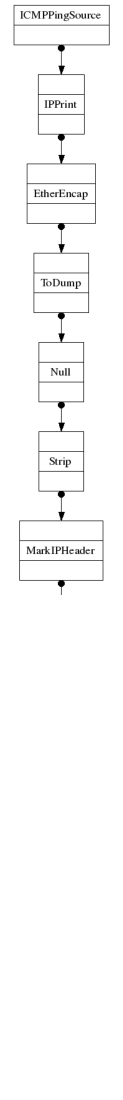
\includegraphics[width=1cm]{figures/clickvizcropped.pdf}
\end{figure}
\end{minipage}

\end{frame}
% subsection click_viz (end)

\subsection{gdb} % (fold)
\label{sub:gdb}

\begin{frame}
\frametitle{Gnu Debugger}
A low-level, well known and very powerful debugger

Basics:
\begin{itemize}
	\item \lstinline!gdb userlevel/click!
	\item \lstinline!run someclickscript.click!
	\item (wait for crash)
	\item \lstinline!bt!
	\item \lstinline!quit!
\end{itemize}
\end{frame}
% subsection gdb (end)

\subsection{valgrind} % (fold)
\label{sub:valgrind}

\begin{frame}
\frametitle{valgrind}
A memory debugger, shows and debugs invalid memory access

Basic usage: \lstinline!valgrind userlevel/click somescript.click!

Errors and warnings might come from glibc or Click elements, and might appear in other elements.
\end{frame}
% subsection valgrind (end)

\section*{Acknowledgements}
\frame{
A big thank you to Michael Voorhaen, one of the original authors of these slides.
}
\end{document}


